\documentclass[runningheads]{llncs}

\usepackage{graphicx}

%
%%% Used for displaying a sample figure. If possible, figure files should
%%% be included in EPS format..
%%% If you use the hyperref package, please uncomment the following line
%%% to display URLs in blue roman font according to Springer's eBook style:
%%% \renewcommand\UrlFont{\color{blue}\rmfamily}
%
\begin{document}
%%%\title{Tecnicas y Herramientas Modernas\thanks{Supported by organization x.}}
\title{Indicadores de Energia Sustentable}
%
%%% \titlerunning{Abbreviated paper title}
%%% If the paper title is too long for the running head, you can set
%%% an abbreviated paper title here
%

\author{Pedrosa %\inst{1}
\and
Galarraga%\inst{2,3}
\and
Carrión
\and
Palma J.C.
\and
Sanchez
\and
Portabella
\and
Ruoti
\and
Puelles
\and
Llampa
\and
Niscola 
\and
Romero
\and
Plaza
\and
Acquistapace}
%
\authorrunning{Los Absorbedores
\and
Lady Gilbert}
%
%%% First names are abbreviated in the running head.
%%% If there are more than two authors, 'et al.' is used.
%
\institute {Facultad de Ingeniería, Universidad Nacional de Cuyo} 
%\email{lncs@springer.com}\\
%\url{http://www.springer.com/gp/computer-science/lncs} \and
%
%ABC Institute, Rupert-Karls-University Heidelberg, Heidelberg, Germany\\
%\email{\{abc,lncs\}@uni-heidelberg.de}}
%
\maketitle              
%typeset the header of the contribution
%
\setcounter{section}{6}

%%Reni%%%
\begin{abstract}En este capítulo se presentan distintas organizaciones internacionales que realizan métricas asociadas a la preservación ambiental. Posteriormente se introducen disciplinas y herramientas asociadas a este propósito, tales como el LCA (análisis del ciclo de vida) o la ecología política. Por último, se analizan las distintas interpretaciones que actores sociales (gobiernos, empresas, instituciones) tienen la capacidad de imponer y las consecuencias en la sociedad.

%%%Reni%%%
\keywords{Ecología industrial \and Evaluación de riesgos \and LCA \and Ciclo de vida \and GHG \and Análisis de vulnerabilidad \and Políticas}
\end{abstract}


\subsection {Ecología Industrial}
\keywords{Ecología industrial \and contaminacion \and sinergia}
\bigskip
La ecología industrial es un enfoque para repensar los sistemas de producción a fin de minimizar los desechos sobre la base de diseños que imitan a los ecosistemas, donde los desechos se convierten en materia prima o insumos para otros procesos. La investigación en ecología industrial es a menudo exploratoria y descriptiva, una metáfora de cómo los sistemas de producción podrían integrarse (Ehrenfeld 2004). La idea subyacente de la ecología industrial es ir más allá de las soluciones de contaminación para replantear radicalmente los procesos de producción, prevenir la contaminación y perseguir la producción ambientalmente benigna. El objetivo de este replanteamiento radical ha llevado a la exploración del concepto de simbiosis industrial, en el que las instalaciones que dependen de recursos compartidos e interconectados se ubicarían conjuntamente para maximizar las eficiencias y sinergias.

\paragraph{Definición}La ecología industrial es una metáfora utilizada para describir sistemas industriales que no generan residuos porque los procesos utilizan a estos como insumos o materias primas para otros procesos industriales.

\bigskip   
La investigación en ecología industrial es de naturaleza "exploratoria y descriptiva". El concepto establece una visión de simbiosis entre los sistemas de producción. Las cuatro leyes de la ecología establecen unas cuantas reglas para pensar en la producción eco-industrial: (1) todo debe ir a alguna parte, (2) todo está interconectado, (3) la naturaleza sabe mejor, y (4) no hay almuerzos gratis en la naturaleza (Plebeyo 1971). Estos principios se han aplicado a varios parques eco-industriales diseñados para interconectar sinérgicamente los sistemas industriales para aprovechar los productos de desecho y otros recursos compartidos.

\bigskip
Un buen ejemplo lo encontramos en Kalundborg, una localidad de unas 20.000 personas situada al norte de Dinamarca. Este modelo de ecologia industrial se implemento hace años, y poco a poco ha ido mejorando y creciendo, hasta lo que hoy en dia es uno de los entornos de ecologia industrial mas eficientes de Europa.

\bigskip
Kalundborg cuenta con un parque ecoindustrial que funciona igual que una cadena trófica de un ecosistema natural.
En Kalundborg hay: una planta de electricidad; una refinería de petróleo; una fábrica de ácido sulfúrico; una cementera; una fábrica de cartón yeso; una fábrica de biomasa; granjas locales.

\bigskip
Además, también se fabrican y reparan las carreteras, así como se dota de servicios a la propia ciudad de Kalundborg. Lo realmente interesante de todo esto es que, todos estos edificios y sus actividades están relacionadas entre sí.

\begin{figure}[htbp] % La H es de Here
  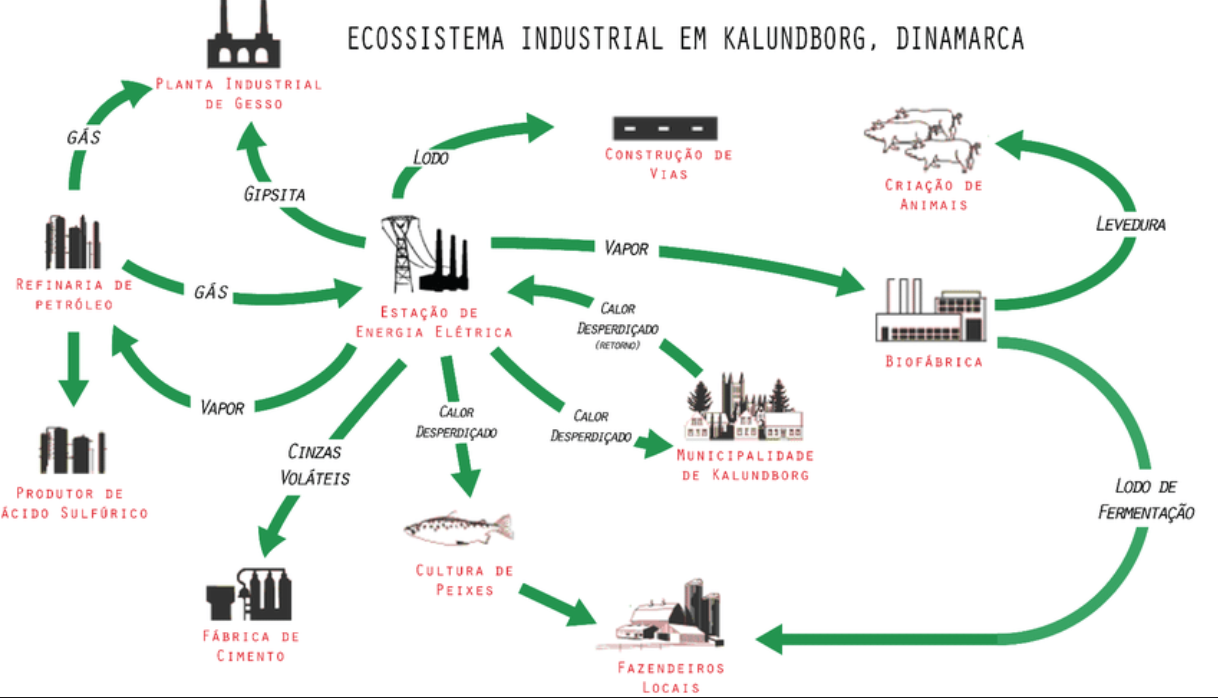
\includegraphics[width=\textwidth]{Parque.png}
 \caption{Ecosistema industrial en Kalundborg, Dinamarca }
 \label{Parque}
\end{figure}

\subsection{Indicadores de sustentabilidad}

\keywords{Indicadores de Sustentabilidad \and  responsabilidad social corporativa \and RSC}
\bigskip
El cambio ambiental global está empujando límites planetarios para algunos impactos, incluido el clima, las cargas de nitrógeno y la biodiversidad. El objetivo de desarrollar indicadores de sustentabilidad es contar con medidas cuantitativas que representen el impacto de las actividades humanas para que sea posible comprender el enfoque más holístico o determinar el proceso menos impactante.

\bigskip
La investigación de indicadores de sustentabilidad ha despegado en los últimos años a medida que la información sobre responsabilidad social corporativa (RSC) ha aumentado. A su vez este tipo de métricas se integran en las políticas públicas y las revelaciones públicas sobre el desempeño ambiental. A medida que los indicadores de sustentabilidad han crecido en popularidad, gran parte de la conversación se centra ahora en cómo armonizar y estandarizar los enfoques de medición ambiental (Hopwood 2009). Los esfuerzos están dirigidos a entender cómo estandarizar cómo se mide, enumera y codifica la sustentabilidad en conjuntos de métricas de desempeño. Las historias y los legados institucionales pueden dar forma a la estandarización y la contabilidad ambiental y revelar cómo se construyen socialmente y se incrustan con suposiciones sobre el mundo (Heiskanen 1999).

\bigskip
Entre las principales organizaciones que preparan información sobre sustentabilidad, figura la Iniciativa Mundial de Presentación de Informes (GRI). Los indicadores incluyen emisiones de calidad del aire (contaminantes del aire, metales pesados, compuestos orgánicos volátiles), uso y eliminación de agua, gases de efecto invernadero, efluentes de nitrógeno, y cientos de otros indicadores. La consideración crucial en el desarrollo del indicador es obtener el impacto correcto en el numerador y la unidad de actividad o salida correcta en el denominador.

\subsection{Huella de carbono}
\keywords{Huella de Carbono \and normas ISO \and GEI (gases de efecto invernadero)} 
\bigskip
La mayoría de las actividades cotidianas de las personas involucran emisiones de carbono. Estas contribuciones en las naciones industrializadas son mayores que las que ocurren en los países en desarrollo, aunque el crecimiento es cada vez más rápido en ellas. Se observan  diferencias también en los lugares con diferentes hábitos culturales.

\bigskip
Los creadores del GEI (gases de efecto invernadero) hacen uso de estas emisiones tanto para desarrollar políticas nacionales de carbono y energías renovables, como también para que la gente conozca su aporte de emisión y sean conscientes y hagan algo al respecto para reducirlas.

\bigskip
La huella de carbono analiza distintos patrones y comportamientos de consumo individual como calefacción, desplazamientos, etc. y estima la contribución de cada individuo, organización o país, para luego sacar un total.

\bigskip
Hay estándares internacionales para la realización de la huella de carbono como la norma ISO y numerosas entidades como el Proyecto de Divulgación de Carbono y la Iniciativa Mundial de Presentación de Informes. Los estándares establecen las reglas clave para generar supuestos o tomar decisiones de cómo asignar impactos y emisiones.
La huella de carbono varía entre 1 a 100 toneladas métricas anualmente y probablemente haya casos de mayor aporte.

\bigskip
Los científicos dicen que para mantener las emisiones individuales dentro de un valor razonable, para dejar de contribuir tanto al calentamiento global, los números deberían ser de 2 toneladas métricas anuales de CO2 por persona.

\bigskip
En la Argentina, en junio del año 2020, investigadores de la Argentina, Perú y España midieron la huella de carbono en establecimientos ganaderos dedicados a la producción de carne de cordero y de lana. La produccion de ovejas en los establecimientos seleccionados representaron el 75 al 90 cada cien de las contribuciones, seguido del procesamiento en la industria del 2 al 15 cada cien y las del transporte a la industria oscilaron entre un 3 y 15 cada cien, dependiendo de la distancia de las instalaciones de procesamiento. Los resultados obtenidos de HC dan valores para fijar objetivos de mitigacion y medir el progreso, ademas de dar referencias para el etiquetado de carbono en productos alimenticios.

\subsection{Evaluación del ciclo de vida}
\keywords{Ciclo de vida, sustentabilidad \and diseño verde  \and ecologia industrial  \and efecto invernadero  \and impacto ambiental  \and materia prima fotovoltaica  \and LCA} 
\bigskip
 Existe una tendencia creciente hacia la medición de los impactos ambientales de los productos básicos, lazos y sistemas de producción, utilizando la evaluación del ciclo de vida (LCA) y utilizando estos métodos para informar el desarrollo de estándares de sostenibilidad. Este marco contable ambiental está transformando la forma en que se gobiernan algunos sistemas de productos básicos, a medida que se convierten en parte integral de la formulación de políticas e influyen cada vez más en los procesos de producción. LCA es una herramienta para promover conceptos clave en estudios de sustentabilidad, diseño verde y ecología industrial. Es un enfoque cuantitativo utilizado por los profesionales para explorar los impactos materiales de ciertas relaciones socioecológicas: el trabajo, las comunidades y paisajes, aunque se reducen a números, es importante que se mantengan los datos en contexto.

\bigskip
La LCA parece ser un marco contable objetivo en la superficie y por lo tanto, apolítico, pero también requiere actos de conmensurabilidad. Cuantifica y califica las huellas de carbono, efecto invernadero, inventarios de gas, tóxicos y recuperación de energía, entre otras categorías de impacto.

\bigskip
Los dos tipos de ACV clave son "atribucionales vs consecuentes". Los atribucionales esencialmente catalogan todos los materiales y les asigna emisiones, mientras que los consecuentes preguntan además cuáles son las consecuencias de producir ese producto.

\bigskip
La LCA destila los impactos en una métrica cuantitativa. Por ejemplo, una calculadora de huella de carbono informa las emisiones de carbono del ciclo de vida en toneladas o libras de carbono. Algunos estudios de transporte informan costos sobre el costo por distancia como un aproximado del uso de energía. Las LCA más sólidas "normalizan" los datos en función de varias métricas para asegurarse de que las medidas calculadas, utilizando un conjunto de unidades, no oscurezcan los resultados.

\subsubsection{Definición de objetivos y alcances}

\bigskip
Al establecer el objetivo y alcance, es importante pensar en las motivaciones y disponibilidad de datos y garantizar exactamente lo que desea hacer, definido claramente al comienzo. Aquí, es fundamental definir términos, métricas, identificar fuentes de datos y análisis de la calidad, esencialmente planificando el conjunto completo de herramientas que se utilizarán en el análisis. Piense en los resultados que desea ver al final: contaminantes del aire, agua, efluentes, emisiones peligrosas y gases de efecto invernadero. ¿Cuales son las cartas y gráficos? ¿Cuáles son las categorías o variables que le gustaría comparar?

\bigskip
Una decisión importante en esta etapa es establecer los límites del sistema. ¿Cuáles son los usos finales? ¿Dónde comienza y termina este producto? ¿Hasta qué punto debe ascender la cadena de suministro?¿Nosotros contamos? ¿Qué operaciones importantes deben incluirse? ¿Cómo deberían asignarse los coproductos? ¿Cuál es el alcance de la geografía? ¿De dónde provienen los datos? ¿Datos nacionales?¿Datos regionales? ¿Datos de origen privado? Un desafío importante de la LCA es la transmisión de datos clásica, que puede ser muy antigua en algunos casos. Peor aún es no tener ningún dato y confiando en algunas reglas generales basadas en algunas de las ideas básicas detrás de un proceso en lugar de usar un proxy. Por ejemplo, si el proceso es exotérmico y requiere calentamiento, se podría estimar este requerimiento de energía. Si los requisitos energéticos para hacer un cierto tipo de plástico no está disponible, puede ser conveniente utilizar un producto similar.

\subsubsection{Inventario del ciclo de vida}
\begin{itemize}
    \item Inventario del ciclo de vida
    \item Evaluación del impacto del ciclo de vida
    \item Interpretación del ciclo de la vida, conclusiones y recomendaciones para el manejo del ciclo.
\end{itemize}

\bigskip
Hay una tendencia creciente hacia la medición del impacto ambiental generado por la producción de bienes y servicios utilizando el Life Cicle Assessment (LCA), y el uso de estas medidas para informar del desarrollo de estándares sostenibles. En este marco de contabilidad ambiental está transformando la manera en que algunos sistemas de producción son gobernados, en la medida que se van convirtiendo en partes integrales en la creación de políticas y métodos de producción acorde. Sin embargo, si bien LCA es una herramienta crítica para el avance de conceptos claves en los estudios de sustentabilidad, diseño ecológico, y ecología industrial, el abordaje cuantitativo usado por los especialistas tiende a eliminar las relaciones socio-ecológicas –el trabajo, las comunidades, y los paisajes– que constituyen esta cadena de bienes y servicios. Esto significa que los esquemas como el LCA  tienen un alcance limitado en cuanto a la distribución del impacto –en cuestiones relacionadas con la justicia medioambiental. Medidas derivadas del LCA pueden tener asociada una agencia política basada en números, porque los números son “científicamente correctos”. 

\bigskip
Este capítulo repasa sobre diversos estudios del ciclo de vida y justicia mediambiental relacionados con la cadena de materias primas fotovoltaicas, donde el LCA se ha convertido en una norma política e industrial y donde una robusta comunidad de expertos en LCA ha surgido durante los últimos 30 años, buscando darle forma a la sustentabilidad del ciclo de vida fotovoltaico. 

\bigskip
Las herramientas de LCA y los modelos en particular tienen un rol fundamental “no en solucionar problemas sino en construirlos pero de una manera distinta” (Heiskanen, 2002). Como remarcó Stone, “contar incluye juicio sobre inclusión y exclusión” (Stone, 2002). Entonces, la creación de cualquier métrica incluye la delimitación de fronteras alrededor de los que se debe incluir, y lo que no. 

\bigskip
Las categorías de impacto usadas en LCA incluyen el potencial de calentamiento global, reducción de la capa de ozono, materia particulada, smog fotoquímico smog químico; eutrofización; toxicidad por ecotoxicidad terrestre/acuática; toxicidad humana (años de vida perdidos); acidificación; agotamiento de los recursos abióticos; y huellas de agua azul, verde y gris (Fthenakis et al. 2008).

\bigskip
Podría decirse que el aspecto más débil del uso de LCA en las políticas son los elementos subjetivos del proceso a lo largo de LCA: juicios sobre qué incluir, excluir y cómo medir. Sin embargo es la fase de interpretación la que propone un desafío porque se basa en la comprensión de los sistemas y en cómo poner los hallazgos de LCA en contexto.

\subsection{Retorno de energía en inversiones}
\keywords{ EROI (energy return on investment) \and inversiones \and energía}
\bigskip
Una medida clave para entender el balance de energía de diferentes fuentes y tecnologías es el retorno de energía en inversiones EROI (energy return on investment). Podemos hacer una analogía con inversiones financieras: el EROI es el factor que multiplica a la inversión para obtener el retorno esperado. Ahora volviendo a términos de energía, los EROI son importantes debido a que pueden revelar pérdidas o ineficiencias que no son del todo evidentes. Por ejemplo, una unidad de energía rinde 7 unidades de combustible, mientras que una unidad de energía puede que rinda solo 3 unidades del etanol.

\bigskip
Las investigaciones en la producción de etanol revelan que el EROI de la producción de etanol a partir de maíz va desde 0,75 a 1,7. Esto se debe mayormente al uso de fertilizantes en la producción del maíz, y a los combustibles para calefacción en algunas instalaciones. Otros granos pueden tener un EROI mayores del orden de 10. Más allá de eso, los límites de la radiación solar, desafían para obtener mayor energía de la misma. Si el terreno no fuera una restricción, un sistema fotovoltaico permitiría obtener más energía por hectárea.

\bigskip
Los EROI de los sistemas fotovoltaicos son medidos en un rango de 10 a 22 años. Un artículo de divulgación provocativo aclama que la industria fotovoltaica consumió solamente de energía eléctrica hasta 2010. Luego de eso comenzó a producir más energía de la que invertía para producir más dispositivos. De aquí en adelante, la energía solar salvó sus deudas con GHG (Greenhouse gas) emitido por manufactura, cadena de suministros y otros segmentos de la cadena.

\subsection{Tiempo de devolución de la energía}
\keywords{Inversiones \and energía \and paneles fotovoltaicos}

\bigskip
El tiempo de devolución de la energía EPT (energy payback time) nos permite visualizar el tiempo esperado para comenzar a ver retornos de las inversiones iniciales y ciclo de vida de la energía. Los paneles solares fotovoltaicos comúnmente requieren un tiempo para recuperar la energía invertida en la manufactura y transporte. Este tiempo varía entre seis meses a dos o tres años para silicio cristalino.

\begin{figure}[htbp] % La H es de Here
  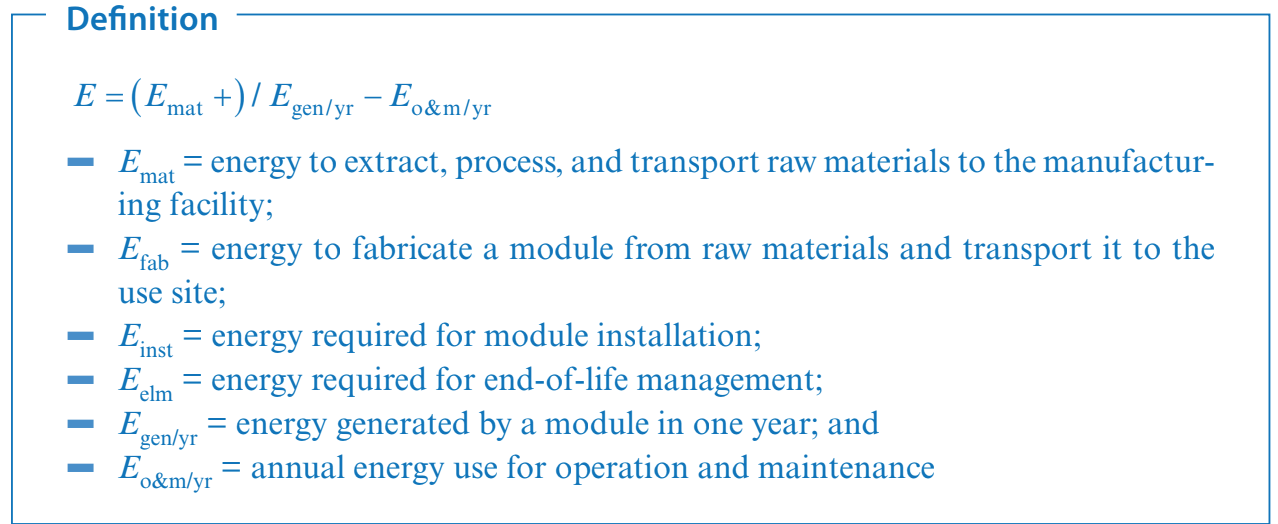
\includegraphics[width=\textwidth]{Definition.png}
 \caption{Cálculo de las distintas energías}
 \label{Definition}
\end{figure}

\bigskip
Analogamente se podría utilizar otra entrada de acuerdo con esta idea y producir tiempo de recuperación de GEI, y así sucesivamente. Aqui, la contabilidad sería similar excepto que en lugar de inversiones en energía a lo largo del ciclo de vida, se podría medir la entrada de emisiones de GEI en el sistema de productos básicos y el tiempo de equilibrio con los ahorros de GE.

\subsection{Marca de agua}
\keywords{Agua \and huella hídrica \and potabilidad.}
\bigskip
Los datos sobre aguas residuales se utilizarán para desarrollar huellas azul, verde e hídrica y compararlas con la producción actual. Las huellas hídricas son indicadores que representan impactos en los recursos hídricos por un estimativo de las cantidades de agua, además de los impactos en la calidad del agua. Este nos permite dividir el agua en 3 componentes.

\bigskip
 Inicialmente, la huella de agua azul evalúa el volumen de agua subterránea y superficial extraída, eliminada o consumida del ciclo hídrico que se utiliza para producir. Ya que las fuentes de agua libre son limitadas, esta es la técnica más convincente y directa. Porque refleja con mayor precisión la cantidad de agua utilizada.
 
 \bigskip
 Luego, la huella hídrica gris es un indicador de la contaminación del agua y la definimos como la cantidad de agua necesaria para contrarrestar la contaminación del agua a su origen o a un estándar aceptable (Mekonnen y Hoekstra 2011). La evaluación del agua gris requiere un exámen de dos pasos. El primer paso es estimar un factor de dilución, lo que requiere evaluar el origen de calidad del agua (limitación de aguas residuales o un estándar de agua potable) que determine en qué grado el agua está contaminada. En segundo lugar, requiere una medida o evaluación del grado de contaminación del agua. Con el conocimiento de estos dos pasos, podemos estimar el factor de dilución.

%%%%aca otra pagina  155

\bigskip
Con un factor de dilución conocido, se puede dar una estimación de la huella hídrica gris con una combinación de información de la cantidad de agua eliminada y normalizada por la cantidad de producción de gas natural.
 
 
 
 %%%% otra pagina 156
 
\bigskip
la huella hídrica verde es el "uso del flujo que se evapora de la superficie terrestre" (Mekonnen y Hoekstra 2011,1577). Las huellas hídricas verdes son aplicadas principalmente a productos de la agricultura o  de la forestación.

\bigskip
La huella hídrica verde es una medida de la pérdida de agua por evaporación durante la fotosíntesis. Se utiliza en productos y procesos agrícolas principalmente. Para tener una imagen completa de los impactos del agua, los indicadores de calidad del agua son esenciales.  Además, hay una gran diferencia si el cuerpo de agua que recibe el producto ya está dañado, protegido o si requiere alguna consideración. Varios indicadores importantes del agua son nitrato, un concentrado de fósforo en el río, arroyo o lago receptor, medido en miligramos por litro (mg/L). Esto también es afectado por la elección del cultivo y su porcentaje de residuo. La cantidad de fertilizante nitrogenado aplicado; que puede causar eutrificación e hipoxialidad; y afecta la potabilidad del agua, ya que la contaminación por nitrógeno está relacionada con problemas que afectan a las comunidades de trabajadores agrícolas en US, por ejemplo, el síndrome del bebé azul. Otros indicadores claves son sólidos en suspensión en arroyos, que también se ven afectados por los factores anteriormente nombrados. Estos afluentes pueden causar impactos bentónicos y provocar sedimentación en los cuerpos de agua.

\bigskip
Finalmente, medir la concentración de pesticida en mg/L, también ayuda a comprender si hay exposición a sustancias químicas cancerígenas. El uso de pesticidas también es afectado por la elección del cultivo y la labranza.
 

\subsection{Pensamiento Cradle-to-Cradle}
\keywords{Producción \and sustancias químicas peligrosas \and sustentabilidad}
 
 \bigskip
Los dopantes se utilizan para cargar semiconductores y son suministrados por empresas especializadas. La soldadura y la cinta son piezas clave necesarias para interconectar un módulo fotovoltaico. El ácido clórico es un insumo importante para su fabricación. La hoja es un material polimérico que protege las células fotovoltaicas. El encapsulante es un material polimérico fijado encima del vidrio en un PV para protegerlo de la humedad.

\bigskip
La caja de conexiones es la interfaz de interconexión entre la electricidad generada por los módulos y el sistema eléctrico. Por lo general se encuentra en la parte posterior del módulo. En la mayoría de las aplicaciones la caja de conexiones está conectada a un inversor, que luego se enruta a la caja eléctrica en una casa. 

\bigskip
Reciclaje, reutilización y desmaterialización son conceptos de diseño que funcionan contra el desperdicio, el agotamiento de los recursos y la obsolescencia programada \ref{hola2}.

\begin{figure}[htbp] % La H es de Here
  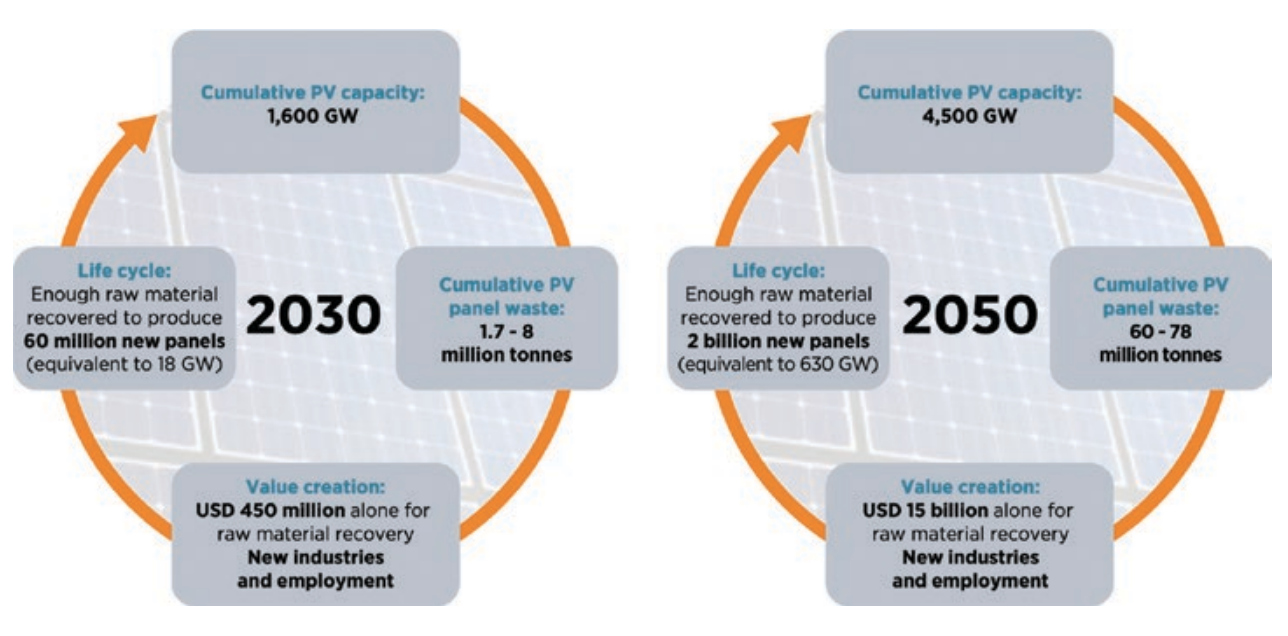
\includegraphics[width=\textwidth]{hola2.png}
 \caption{Reciclaje de fotovoltaicas al final de su vida útil, puesta en valor}
 \label{hola2}
\end{figure}

\subsection{La transición a una industria sostenible}
\keywords{ Industria química}
\bigskip
Con la llegada del siglo XXI, la producción es cada vez más prominente. Los defensores de este enfoque citan dos razones. Primero, la producción está asociada con impactos ambientales "insostenibles". Muchos productos son reconocidos por contener sustancias químicas tóxicas, persistentes o bioacumulativas. Su uso, almacenamiento, transporte y deterioro con el tiempo pueden conducir a la disipación en el medio ambiente. Si la industria quiere lograr una mayor sostenibilidad, necesita reconsiderar sus opciones de producción. A pesar de los avances en el desarrollo de principios de química sostenible, durante la década de 1990, entre otros desarrollos, la producción química sigue siendo un área de confusión para la industria, los ciudadanos y los gobiernos en Europa y los EE. UU. La UE ha adoptado una "política de productos integrada" y la eliminación gradual de algunos productos químicos peligrosos. Generalmente, los gobiernos son reacios a supervisar la producción debido a que afectaría el poder de la industria. La UE ha creído que el compromiso de los ciudadanos, los consumidores y los grupos medioambientales en productos y el diseño de procesos no son factibles en gran medida. Por lo tanto, la industria puede enfrentar menos escrutinio de sus prácticas de producción, incluida la adopción de prácticas que buscan diseño de procesos intrínsecamente más seguros

\bigskip
Se está observando, en base a distintos estudios, que diferentes áreas de las empresas están empezando a tener en cuenta el concepto de sustentabilidad, empujados por los entes reguladores, las necesidades de las compañías y los consumidores, teniendo estos últimos la mayor influencia para fomentar el cambio. Pero todas estas nuevas ideas dependen, en su mayoría, de la interpretación de la propia empresa sobre el concepto de sustentabilidad, lo que no otorga una noción estándar general para todos.

\bigskip
Al no tener una regulación más detallada y amplia las industrias generan su propia idea de sustentabilidad, la que puede no ser compartida por otros. Un ejemplo es la industria química, la cual puede cambiar el tipo de materias primas que ellos consideran menos contaminantes, pero lo siguen siendo para muchos otros.  Muchas veces ocurre que cambian elementos cuyos estudios determinaron un impacto negativo en el medio ambiente por otros de los cuales no se tiene tanta información, por lo que no están prohibidos; no por que no sean peligrosos sino porque no se tiene la información suficiente sobre ellos.
Hoy en día hay distintas instituciones que están buscando generar estándares sostenibles a partir del estudio y análisis de múltiples componentes clave.

\subsection{Química verde}

\bigskip
La química verde es un “área de investigación en estudios sustentables” cuyo objetivo es mejorar las prácticas dentro de la industria química y hacerla más sostenible frente a otras que solo buscan reducir los peligros de las técnicas actuales. Además, busca incluir puntos de vista más variados, como las implicaciones políticas y sociales.

\bigskip
La importancia de la industria química radica en la gran variedad de actividades que dependen de ella, tanto de productos químicos en si o como la industria cosmética, de juguetes o la industria energética.
La química verde busca generar alternativas que no solo cambien las propuestas actuales sino también que las mejoren y las hagan más eficientes.

\subsection{Ecología: Política – Industrial}
\keywords{Análisis del ciclo de vida \and impacto ambiental \and ecología política-ambiental
}

\bigskip
El concepto de ecología empieza a ser tenida en cuenta en diferentes instituciones gubernamentales; dentro del mismo podemos encontrar términos como “LCA” que hace referencia a la “evaluación del ciclo de vida”.  Esta busca comparar distintos aspectos de la industria como el tipo de energía que utiliza, las emisiones de CO2, o desechos fluviales que genera. Estos conceptos buscan ser un criterio estándar internacional para el futuro desarrollo, impulsado también desde un frente político.

\bigskip
Una vez terminado el inventario y el análisis LCA se necesita un analista que procese los datos. ¿Cómo se puede aplicar la LCA en la transición de carbono sostenible sin reducir la calidad del producto? Actualmente la sociedad observa seriamente las aplicaciones de LCA, ya que se han vuelto de carácter económico, político y social.

\bigskip
En la literatura revisada por la comunidad, el LCA se emplea ampliamente para comparar sistemas energéticos. La aproximación sistemática y cuantitativa del LCA le permite considerar los impactos ambientales de la energía debido a que puede comparar fácilmente los recursos energéticos (Espeland and Stevens 1998). La energía es una demanda derivada, es decir, la demanda de servicios energéticos es un intermediario para la demanda de recursos energéticos. Le red eléctrica requiere administrar un complejo sistema de centrales eléctricas y demandas de electricidad de varios consumidores, haciendo dichas comparaciones de recursos eléctricos no sólo posibles sino que también importantes para las políticas ambientales y climáticas. La gente quiere que las salidas de corriente funcionen al igual que los autos, no les interesa qué recursos lo hacen posible. Esto significa que la energía se compara mediante unidades funcionales; toda energía puede convertirse en otras unidades empleadas para representar energía (kilowatt-hora, megajoules, barriles de petróleo equivalente, etc.). Existen más LCAs escritos en inglés sobre sistemas energéticos que sobre cualquier otra industria o sector. Búsquedas en bases de datos durante abril de 2016 entregaron 104.000 resultados para "evaluación del ciclo de vida" más "energía" en Google Scholar y la misma búsqueda en Science Direct ofreció 115.170; búsquedas similares para "evaluación del ciclo de vida" más "alimento" (86.160 Science Direct) y "agricultura" (38.900 Google Scholar; 31.185 Science Direct) devolvieron resultados similares. Es posible que no exista un grupo comparable de LCAs específicos de cada industria bajo una amplia armonización, y el LCA se está incorporando en muchos instrumentos reguladores, lo que en los Estados Unidos incluye estándares de rendimiento basados en LCA impuestos por la Agencia de Protección Ambiental y el Departamento de Energía.

\bigskip
Realizar un LCA requiere seguir una serie de pasos, no obstante, estos son procesos iterativos con constantes ajustes, modificaciones y búsquedas de datos. La primera etapa es establecer el objetivo y el alcance del LCA. Donde el investigador o cliente define los parámetros más importantes de ciclo de vida, lo que asegura que la aproximación logre los objetivos del proyecto y sus expectativas al confirmar la unidad funcional, estableciendo límites del sistema, e identificando categorías de impacto ambiental. Estas categorías incluyen potencial de calentamiento global, eutrofización, acidificación, toxicidad, formación de ozono/smog al nivel del suelo, merma del ozono en la estratósfera, agotamiento de los recursos naturales, contaminación del agua, uso de agua, eco-toxicidad, y toxicidad humana. Existen algunas organizaciones que normalizan los datos obtenidos para cada categoría, incluida TRACI

\bigskip
Debido a que las métricas medioambientales cargan con el poder de los números, tienen un efecto discursivo porque se presentan como imágenes imparciales, distanciando lo subjetivo de la política. Basándose principalmente en información cuantitativa el LCA parece objetivo, superando la distancia y la desconfianza (Porter 1995). 
Un LCA es desarrollado en cuatro fases: (1) objetivos y alcance, (2) inventario, (3) evaluación y (4) interpretación. Se debe señalar que a pesar de describir al LCA como una herramienta cuantitativa, dos de las fases centrales son altamente cualitativas.

\bigskip
Hay investigaciones donde se busca entender cómo funciona y cómo están relacionadas distintas áreas, mientras que en el marco del SA buscan cómo pueden estrecharse datos. Pudiendo así obtener ciertas conclusiones.

 %% por si necesitamos poner referencias a una figura(Fig. \ref{La71}) 

%% para poner imagenes
%\begin{figure}%[h] % La H es de Here
 % \includegraphics[width=\textwidth]{La71}
 % \caption{Subestación eléctrica de Amboy Crater, California, en el desierto de Mojave}
 % \label{La71}
%\end{figure}


%\begin{figure}[h] %https://ondiz.github.io/cursoLatex/Contenido/04.Imagenes.html 
 % \includegraphics[width=\textwidth]{La72}
  %\caption{Las ubicaciones de la infraestructura de las líneas de transmisión presentan dificultades y desafíos en áreas con riesgo de incendio o en áreas naturales.}
  %\label{La72}
%\end{figure}


\section*{Conclusión}
Este capítulo desarrolló conceptos claves para  la ciencia y la ingeniería de la sustentabilidad, introduciéndonos a instrumentos de análisis como lo son la evaluación del ciclo de vida, la ecología industrial, la evaluación de riesgos y alternativas, el análisis de la vulnerabilidad y la ciencia del uso de la tierra. Se proponen formas de evaluar los impactos de las tecnologías energéticas, infraestructura y recursos en los sistemas socio-ecológicos de la Tierra. Se busca de esta manera, parametrizar y tener las herramientas necesarias para hacer frente a los desafíos de la humanidad en los años venideros.

\section*{Referencias}
%Hay que referenciar al revisor del trabajo
Alumno revisor: Victoria Palma Cieri

\end{document}